%
% Template for IDIHOM technical reports
%
%  to be processed with pdflatex
%
% based on initial design by K. Hillewaert

\documentclass[12pt,a4paper,a4wide]{article}

% ------------------------------------------------------------------------------
% packages
% ------------------------------------------------------------------------------

% inclusion of non ps-graphics
\usepackage{graphicx,psfrag}
\usepackage{subfig}
\usepackage{epstopdf}
\usepackage{amsfonts,amsmath,amssymb,amscd}
% typesetting headers and footers
\usepackage{fancyhdr}
%\usepackage{lastpage}

% fancy links
\usepackage{color}
\usepackage[citecolor=blue,linkcolor=blue,colorlinks=true]{hyperref}

\usepackage{parskip}
%\usepackage{alltt}
\usepackage{verbatim}
%\usepackage[latin1]{inputenc}
\usepackage{float}
\usepackage{url}
%\usepackage[francais]{babel}
%\def\baselinestretch{2}

%\floatstyle{ruled}
%\newfloat{algorithm}{tbp}{loa}
%\floatname{algorithm}{Algorithm}

\graphicspath{{figures/}}

\renewcommand{\vec}[1]{\ensuremath{\text{\boldmath $#1$\unboldmath}}}
\newcommand{\mvx}{\vec{x}}

% ------------------------------------------------------------------------------
% modify here the properties of the document
% ------------------------------------------------------------------------------

%\newcommand{\reference}{D4.1-30b}
%\newcommand{\shorttitle}{Curvilinear Mesh Generation Capability in Gmsh}
%\newcommand{\theauthor}{T. Toulorge, J.F. Remacle}

\title{Mesh Optimization in Gmsh}
\author{Thomas Toulorge}
\date{November 2014}

% ------------------------------------------------------------------------------
% page title and table of contents
% ------------------------------------------------------------------------------

\begin{document}

% ------------------------------------------------------------------------------
% define headers and footers
% ------------------------------------------------------------------------------

%\pagestyle{fancy}

% header from left to right
%\lhead{\includegraphics[width=0.1\textwidth]{figures/idihom_105px}}
%\chead{}
%\rhead{\small{\textit{\reference~-~\shorttitle}}}
%\renewcommand{\headrulewidth}{0.4pt}

% footer from left to right
%\renewcommand{\footrulewidth}{0.4pt}
%\lfoot{\nouppercase{\leftmark}}
%\cfoot{}
%\rfoot{\thepage/\pageref{LastPage}}
%\newcommand{\chaptermark}[1]{\markboth{#1}{}}

% ------------------------------------------------------------------------------
% main text
% ------------------------------------------------------------------------------

%\newpage
\maketitle


\section{Introduction}

The quality of the meshes generated by Gmsh in a first step is
sometimes not satisfying. The mesh optimization tool aims to
improve the meshes with respect to a given set of quality measures
without performing any topological operation. The tool is designed
to improve locally bad (or even invalid) meshes by using an
optimization algorithm that moves the mesh vertices.


\section{Method}


\subsection{Problem Definition}\label{sec:problem-def}

In order to improve the mesh, an optimization problem is defined:
\[
\min_{\mvx_i} F(\mvx_i)
\]
where the variables $\mvx_i$ are the vertex positions, and the objective
function $F$ takes into account the quality measures of interest. The
position of a vertex in the interior of the computational domain
is normally expressed in terms of its spatial coordinates ($x$, $y$ and
$z$). Vertices classified on a boundary are allowed to move along the
corresponding geometric entity, in case a CAD model is available:
the variables associated to such a vertex are then its parametric
coordinates, as provided by the CAD modeler. Thus, vertices
classified on model edges will have as only degree of freedom the
parametric coordinate $u$, while vertices classified on model faces
will have two degrees of freedom $u$ and $v$. Vertices classified on
a model vertex will not be allowed to move.

The objective function $F$ is the function of all variables $\mvx_i$
to be minimized by moving the nodes. It is the sum of several
\emph{contributions}:
\[
F(\mvx_i) = \sum_{j} F_j(\mvx_i),
\]
where each contribution $F_j(\mvx_i)$ is actually a function of
a \emph{measure} $m_j(\mvx_i)$:
\[
F_j(\mvx_i) = f_j[m_j(\mvx_i)].
\]
A measure is usually a quantity of interest
characterizing the quality or the validity of the mesh (for
instance the scaled Jacobian in high-order meshes). Nevertheless,
a contribution proportional to the square of the node displacement
is often included in the objective function, so that the mesh
remains as similar as possible to the original one, while complying
with other quality constraints.


\subsection{Moving Barriers}

Most often, the mesh optimizer is used to change the mesh so that a
quality or a validity measure lies within a given range of values.
For this purpose, a \emph{log barrier} is used:
\[
f_{\epsilon,\omega}(m) = (m - \omega)^2 +
\log\left(\frac{m-\epsilon}{\omega-\epsilon}\right)^2,
\]
where $\omega$ is the optimal value of the measure $m$, and $\epsilon$
is a value for which the function blows up (cf.
figure~\ref{fig:barrier}). Thus, setting $\epsilon<\omega$ ensures that
the measure $m$ will never drop below the value of $\epsilon$ during the
optimization procedure. Likewise, setting $\epsilon>\omega$ ensures that
$m$ will never exceed $\epsilon$.

\begin{figure}
%\begin{center}
\centering
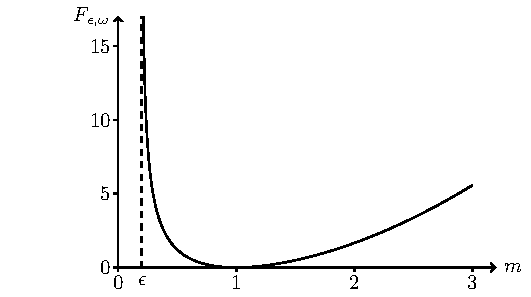
\includegraphics[width=0.45\textwidth]{log_barrier/log_barrier}
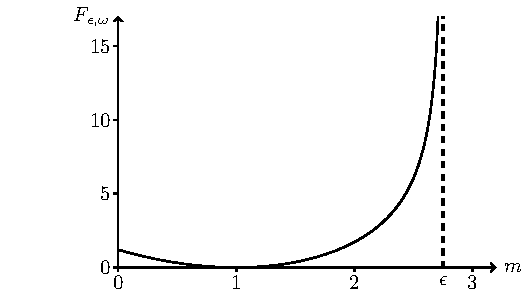
\includegraphics[width=0.45\textwidth]{log_barrier/log_barrier_max}
%\end{center}
\caption{Barrier function for $\omega=1$ and
$\epsilon<\omega$ (left) or $\epsilon>\omega$
(right)\label{fig:barrier}}
\end{figure}

In order for the measure $m$ to remain in the domain of definition of
the barrier function $f_{\epsilon,\omega}$, the value of $\epsilon$ must
be lower than the minimum of $m$ in the domain or subdomain of interest.
Thus, a constraint forcing the measure $m$ to increase to reach a target
minimum value $\bar{\epsilon}$ is introduced through a \emph{moving
barrier}: a sequence of optimization problems is solved. A conjugate
gradient optimization algorithm is applied to each problem, so that $m$
progressively increases. Each run is stopped after a fixed number of
iterations, when stagnation in $m$ is detected, or when the target
criterion $m\geq\bar{\epsilon}$ is reached. Between two runs, $\epsilon$
is reset to a value just below the current minimum value of $m$, so that
the variables remain in the domain of realizability.
Fig.~\ref{fig:opti_process} illustrates this process. The same method
is applied for a maximum constrain.


\subsection{Passes}

It is difficult to handle several moving barriers at the same
time. This is why the optimization procedure can be
used in successive \emph{passes}, between which the objective function
changes. For instance, a moving barrier can be used in a first pass to
bring $m$ to a threshold $m_{\min}$. In a second pass, the objective
function is composed of a fixed barrier set to $m_{\min}$, plus a moving
barrier that forces $m$ to drop below a value $m_{\max}$. This technique
can also prove useful when one wants to impose a constraint on a crucial
measure $m_1$ in a first pass, and then improve another less important
one $m_2$ in a second pass.

\begin{figure}
%\begin{center}
\centering
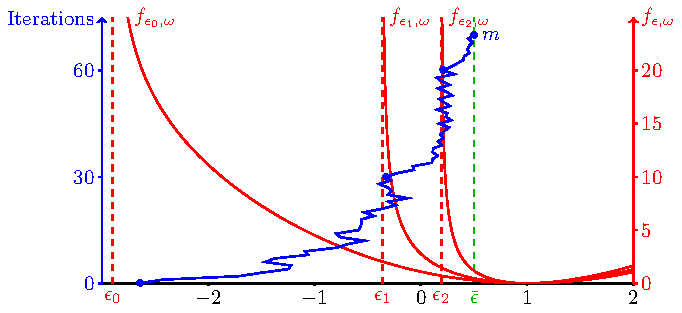
\includegraphics[width=0.95\textwidth]{opti_process/opti_process}
%\end{center}
\caption{Optimization process: three successive series of
(maximum) 30 conjugate gradient iterations\label{fig:opti_process}}
\end{figure}


\subsection{Strategy and Mesh Patches}\label{sec:strategy}

A common use case for the mesh optimization tool is when only a few
small portions of the mesh do not comply with the required quality
criteria. Involving the whole mesh in the optimization process is then
unnecessary, or even prohibitively costly. Therefore, the tool makes it
possible to select \emph{patches} of the mesh (or ``blobs'') in which
the optimization is performed, while the rest of the domain is left
untouched.

The first step in the definition of patches consists in identifying
the mesh elements that do not satisfy the user-defined criteria. A
primary patch containing a user-defined number $N$ of layers of elements
surrounding each ``bad'' element is then built. A geometrical criterion
can also be added: among the elements forming the $N$ layers around the
bad element, only those located within a user-defined distance are
retained. This additional criterion is particularly useful when dealing
with anisotropic meshes, as the boundary layer mesh illustrated in
Fig.~\ref{fig:patches}.
%The optimal values for the number of layers $N$
%and the distance factor are case-dependant: they should involve the lowest
%number of elements while still leaving the optimization procedure enough
%freedom to reach a node configuration that complies with the target mesh
%quality. In complex cases, a unique value of these parameters for the whole
%mesh may lead to patches that are too large at some locations, but too small
%at others. It is then beneficial to use the untangling procedure in an
%adaptive loop where the patch size is progressively increased in case
%the optimization procedure fails to reach the quality criteria.

A potential problem with the patches created as described above is
that they may overlap. Let us consider the case of a subdomain built
around an bad element, that contains another bad element close to its
boundary: this patch may not provide the necessary degrees of freedom
to fix the second bad element, thus the optimization procedure can
fail to reach the mesh quality target in this patch.
In order to avoid such problems, the user can choose between two
strategies:
\begin{description}
\item[Disjoint patches] Overlapping patches are detected and
merged. This strategy ensures that each invalid element in a patch
has enough surrounding elements for the untangling procedure to
be successful, provided the primary patches are large enough, but
it may lead to large patches, which can be computationally expensive.
\item[``One-by-one'' strategy] The untangling procedure is applied
sequentially to each patch, with the objective of fixing only
the invalid element around which it is built, while allowing other
invalid elements in the same patch to remain broken. This strategy
lets the untangling procedure work on small-size patches.
\end{description}

\begin{figure}
\begin{center}
\begin{tabular}{ccc}
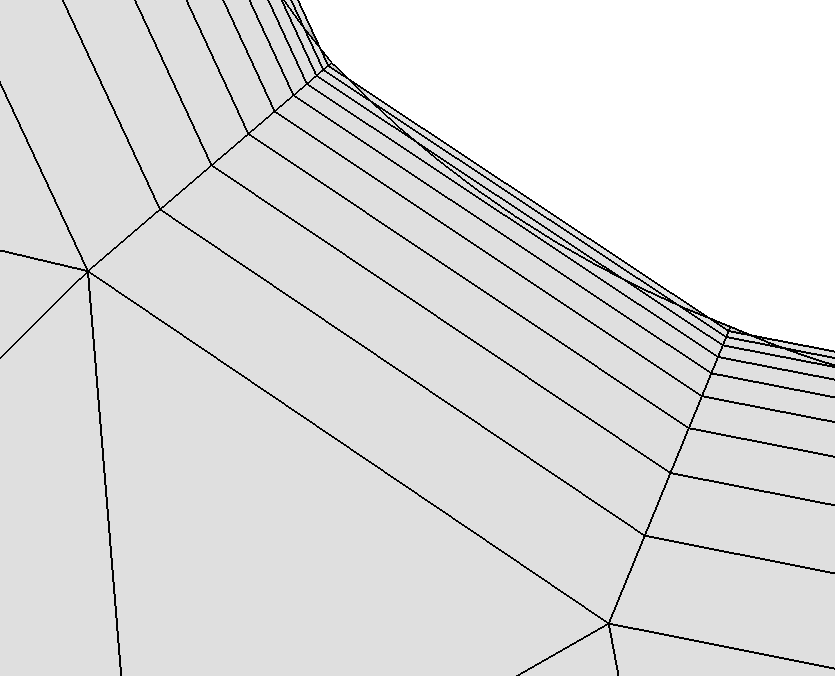
\includegraphics[width=0.33\textwidth]{patches/patch_tangled}&
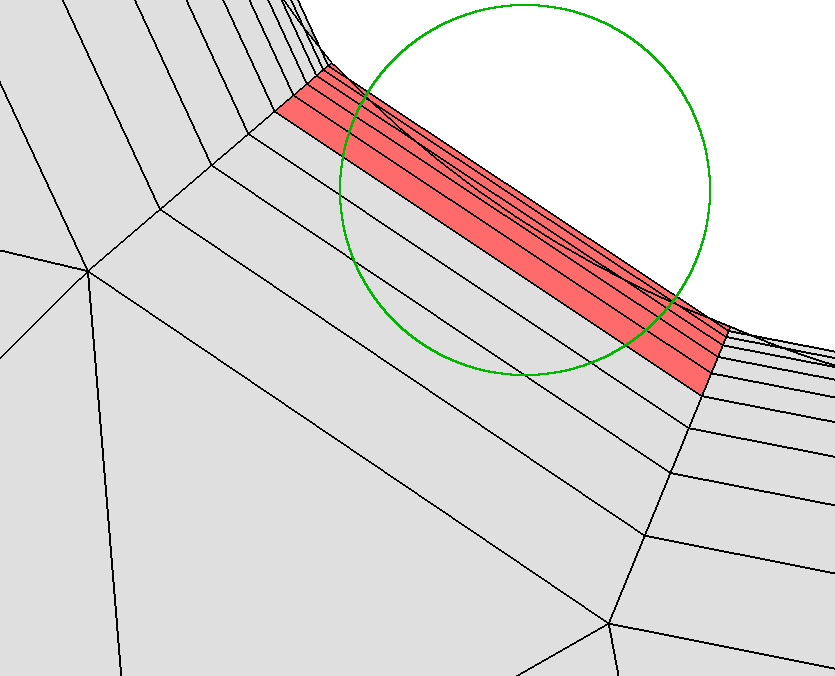
\includegraphics[width=0.33\textwidth]{patches/patch_def}&
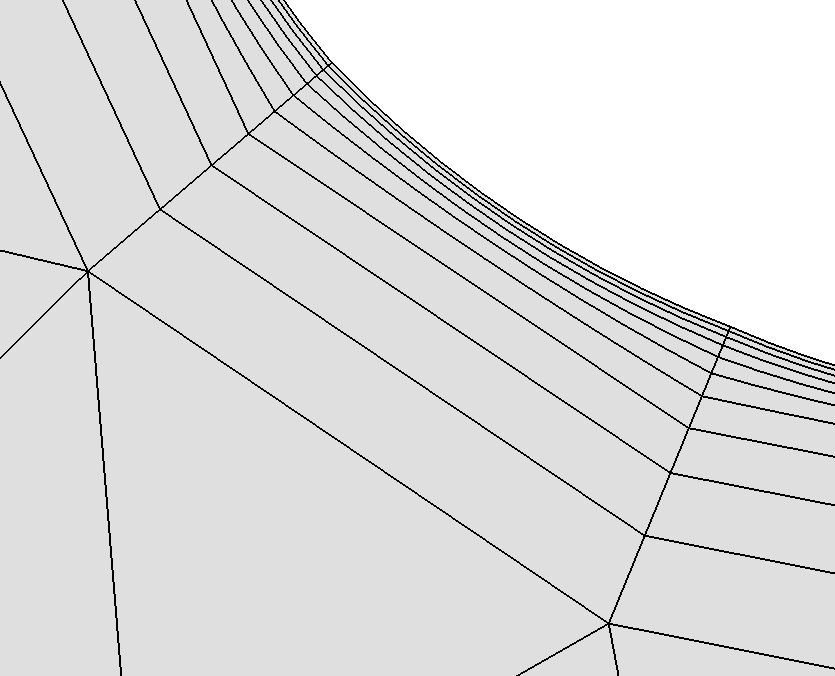
\includegraphics[width=0.33\textwidth]{patches/patch_untangled}
\end{tabular}
\end{center}
\caption{Detail of a boundary-layer mesh on a curved geometry:
tangled quadratic mesh (left), patch definition with $N=5$ layers
in red and geometrical criterion represented by a green circle
(center), untangled mesh (right).
\label{fig:patches}}
\end{figure}


\section{Implementation}


\subsection{General organization}\label{sec:gen-org}

The code of the optimization tool itself is divided into three main
parts:

\begin{itemize}
\item The class \texttt{Patch} handles the information needed from
and provided to the mesh patch, such as the node coordinates and the
value of the quality measures and their gradients. It allows to work
indifferently with physical and parametric node coordinates, and to
avoid modifying the actual mesh data in Gmsh until the optimization
has completed successfully.
\item The class \texttt{MeshOpt} is in charge of setting up and
running the optimization procedure in a given patch. The computation
of the objective function, as well as the assessment of the success
or the failure of the optimization procedure, are handled by classes
that represent each contribution. These classes derived from
\texttt{ObjContrib} are called from \texttt{MeshOpt} through the
class \texttt{ObjectiveFunction}.
\item The function \texttt{meshOptimizer} and the related functions
perform the patch selection and execute the overall optimization
process.
\end{itemize}

In order to tailor the mesh optimization tool to a new application, it
is necessary to carry out the following developments:
\begin{itemize}
\item Implement the main function setting the input parameters (see
Section~\ref{sec:input-param}) and calling the function
\texttt{meshOptimizer}.
\item Implement the class derived from \texttt{MeshOptPatchDef}
that drives the patch selection process (see
Section~\ref{sec:patch-selec}).
\item Implement the classes derived from \texttt{ObjContrib} that
compute the different contributions to the objective function and
check the corresponding criteria (see Section~\ref{sec:obj-func}).
\item Implement the appropriate measure(s) in the class
\texttt{Patch}.
\end{itemize}

These steps are detailed in the following sections.

\subsection{Input Parameters}\label{sec:input-param}

The input parameters that control the optimization process are
provided to \texttt{meshOptimizer} through the structure
\texttt{MeshOptParameters}:

\begin{verbatim}
struct MeshOptParameters {
  int dim ;
  bool onlyVisible ;
  bool fixBndNodes;
  bool useGeomForPatches, useGeomForOpt;
  MeshOptPatchDef *patchDef;
  std::vector<MeshOptPass> pass;
  int displayInterv;
  int verbose;
  int success;
  double CPU;
};
\end{verbatim}

This structure carries the following information:
\begin{itemize}
\item The fields \texttt{dim} and \texttt{onlyVisible} specify the
geometric entities (2D or 3D, all of them or only the visible ones)
in which the mesh will be optimized.
\item The field \texttt{fixBndNodes} determines whether the nodes
located on the boundaries (i.e. the nodes classified on model
entities of dimension \texttt{dim-1}) should be fixed or allowed to
move along their respective model entity.
\item The fields \texttt{useGeomForPatches} and \texttt{useGeomForOpt}
determine whether the geometrical information (i.e. on which model
entity each element is classified) should be passed respectively:
\begin{itemize}
\item to \texttt{patchDef} (see Section~\ref{sec:patch-selec}), in
order to take it into account in the selection of mesh patches,
\item to the classes \texttt{MeshOpt} and \texttt{Patch}, in order
to take it into account in the evaluation of quality measures.
\end{itemize}
If both fields are set to \texttt{false}, the geometrical information
is not computed, which may result in an improved performance.
\item The field \texttt{patchDef} is a pointer on an instance of a
class derived from \texttt{MeshOptPatchDef}, that implements the
methods needed to select the mesh patches (see
Section~\ref{sec:patch-selec}).
\item The vector \texttt{pass} contains instances of the structure
\texttt{MeshOptPass}, which determines the optimization procedure
for each pass, as described hereafter.
\item The fields \texttt{displayInterv} and \texttt{verbose} control
the output (respectively the iteration interval at which the progress
of the Conjugate Gradient procedure is printed to screen and the
overall level of verbosity).
\item The fields \texttt{success} and \texttt{CPU} indicate whether
the overall procedure has been successful (i.e. whether the target
values for the quality measures have been reached) and how much CPU
time it used.
\end{itemize}

The structure \texttt{MeshOptPass}, that specifies the optimization
procedure for each pass, is as follows:

\begin{verbatim}
struct MeshOptPass {
  std::vector<ObjContrib*> contrib;
  int maxOptIter;
  int maxParamUpdates;
};
\end{verbatim}

where:

\begin{itemize}
\item The vector \texttt{contrib} contains pointers on instances
of classes derived from \texttt{ObjContrib}, each instance
describing a contribution to the objective function (see
Section~\ref{sec:obj-func}).
\item The field \texttt{maxOptIter} gives the maximum number of
Conjugate Gradient iterations to be performed for a given objective
function (i.e. before a potential log barrier is moved).
\item The field \texttt{maxParamUpdates} determines the maximum
number of times the objective function is changed, i.e. the number
of times a potential log barrier is moved.
\end{itemize}


\subsection{Patch Selection}\label{sec:patch-selec}

The patch selection process is controlled by an application-specific
class that is derived from \texttt{MeshOptPatchDef}:

\begin{verbatim}
class MeshOptPatchDef {
public:
  enum { STRAT_CONNECTED, STRAT_ONEBYONE };
  int strategy;
  int minLayers, maxLayers;
  union {
    struct {
      int maxPatchAdapt;
      int maxLayersAdaptFact;
      double distanceAdaptFact;
    };
    bool weakMerge;
  };
  virtual ~MeshOptPatchDef() {}
  virtual double elBadness(MElement *el,
                           GEntity* gEnt) const = 0;
  virtual double maxDistance(MElement *el) const = 0;
  virtual int inPatch(const SPoint3 &badBary,
                      double limDist,
                      MElement *el,
                      GEntity* gEnt) const = 0;
protected:
  bool testElInDist(const SPoint3 &P, double limDist,
                    MElement *el) const;
};
\end{verbatim}

The fields of this class contain information about the strategy
and the number of layers in the patch:

\begin{itemize}
\item The field \texttt{strategy} specifies the overall strategy
with (\texttt{STRAT\_DISJOINT} for merging overlapping patches
or \texttt{STRAT\_ONEBYONE} for a sequential treatment, see
Section~\ref{sec:strategy}).
\item The fields \texttt{minLayers} and \texttt{maxLayers} give
respectively the minimum and maximum amount of layers of elements
surrounding the bad element to be included in the patch.
\item Depending on the strategy chosen, additional information
must be provided:
\begin{itemize}
\item If the strategy is \texttt{STRAT\_DISJOINT}, the field
\texttt{weakMerge} specifies whether two patches are merged if
they overlap (value \texttt{false}), or only if a bad element
of one patch is included in the other one (value \texttt{true}).
\item If the strategy is \texttt{STRAT\_ONEBYONE}, an adaptive
process loop is used: the patch size is progressively increased
in case the optimization procedure fails. The maximum number of
adaptations is then controlled by the field \texttt{maxPatchAdapt}.
The growth factor in maximum number of layers and in the maximum
distance criterion at each adaptation is specified by the fields
\texttt{maxLayersAdaptFact} and \texttt{distanceAdaptFact}
respectively.
\end{itemize}
\end{itemize}

Application-specific control of the patch selection is achieved
through the pure virtual methods \texttt{elBadness},
\texttt{maxDistance} and \texttt{inPatch}, that have to be
implemented in a derived class:
\begin{itemize}
\item \texttt{elBadness} determines the ``badness'' of an element:
it returns a negative value for a bad element and a positive value
for a good element. The return value is a floating point instead of
a boolean because the tool always deals with the patches in
decreasing order of badness in the \texttt{STRAT\_ONEBYONE} strategy.
\item \texttt{maxDistance} returns the value the maximum distance
criterion for a given bad element. This value matters only if the
criterion is used in the method \texttt{inPatch}.
\item \texttt{inPatch} determines whether a given element should be
included in a patch. It returns an integer value:
\begin{itemize}
\item $-1$ means that the element should not be included in the patch,
\item $0$ means that the element should be included in the patch only if
it belongs to a layer below \texttt{minLayers},
\item $1$ means that the element should be included in the patch if
it belongs to a layer below \texttt{maxLayers}.
\end{itemize}
This system makes the patch selection very flexible. For instance, it is
possible to exclude unconditionally certain type of elements, or to take
into account certain criteria only in layers between \texttt{minLayers}
and \texttt{maxLayers}. Moreover, the protected method
\texttt{testElInDist} can be called from \texttt{inPatch} for an
efficient test of the distance criterion, if desired.
\end{itemize}



\subsection{Objective Function}\label{sec:obj-func}

As explained in Section~\ref{sec:problem-def}, the objective
function is defined as a sum of contributions, each
contribution being a function of a single measure. In practice,
it is important to follow the progress of the measure to determine
whether the optimization procedure is successful. To this end, the
extrema (minimum and maximum) of the measure over the patch under
consideration are evaluated during the computation of the contribution.
Three criteria are associated to each contribution:
\begin{itemize}
\item A success criterion tests whether the minimum (or maximum)
of the measure is greater (respectively lower) than the target value,
\item A failure criterion tests whether the minimum (or maximum)
of the measure is lower (respectively greater) than a critical value
(for instance the value 0 for the scaled Jacobian in high-order meshes,
below which the mesh is invalid),
\item A stagnation criterion tests whether the minimum (or maximum)
of the measure stagnates compared to the start of the conjugate
gradient algorithm.
\end{itemize}
Thus, a mesh that does not fulfill the failure criterion anywhere can
be considered as acceptable, even if the target has not been reached
in some patches. The stagnation criterion avoids wasting
computation time in problematic cases by stopping an optimization
procedure that does not improve the measure.

As mentioned in Section~\ref{sec:gen-org}, the contributions
are defined by specifying in \texttt{MeshOptPass} a vector of
pointers on instances of classes derived from \texttt{ObjContrib}.
The class \texttt{ObjContrib} is as follows:

\begin{verbatim}
class ObjContrib
{
public:
  ObjContrib(std::string mesName, std::string name);
  virtual ~ObjContrib() {}
  virtual ObjContrib *copy() const = 0;
  const double getMin() { return _min; }
  const double getMax() { return _max; }
  const std::string &getName() const { return _name; }
  const std::string &getMeasureName() const {
    return _measureName;
  }
  virtual void initialize(Patch *mesh) = 0;
  virtual bool fail() = 0;
  virtual bool addContrib(double &Obj,
                          alglib::real_1d_array &gradObj) = 0;
  virtual void updateParameters() = 0;
  virtual bool targetReached() = 0;
  virtual bool stagnated() = 0;
  virtual void updateMinMax() = 0;
  void updateResults();

protected:
  static const double BIGVAL;
  ObjContrib *_parent;
  std::string _measureName, _name;
  double _min, _max;
};
\end{verbatim}

A class defining a contribution should derive from \texttt{ObjContrib}.
One instance should be defined through the constructor in the function
calling the optimization tool, and passed through \texttt{MeshOptPass}.
Then, a new copy of this ``parent'' instance is used for each patch.
\texttt{ObjContrib} stores the pointer to the parent instance
(\texttt{\_parent}), the name of the contribution and the corresponding
measure (\texttt{\_name}, \texttt{\_measureName}) for output purposes, and
the extrema of the measure (\texttt{\_min}, \texttt{\_max}) for the
evaluation of target criteria. The method \texttt{updateResults} updates
the extrema of the measure in the parent instance for reporting purposes.
A derivative class should implement the following methods:

\begin{itemize}
\item The constructor \texttt{ObjContrib} may be needed if fixed
user-defined parameters shall be provided to the contribution (for
instance, a weight factor in the objective function).
\item The method \texttt{copy} returns a new copy of the instance.
\item The method \texttt{initialize} is in charge of initializing
the contribution for each patch, i.e. setting up the fields and
calling the initialization methods of the measure in the class
\texttt{Patch}.
\item The method \texttt{fail} returns whether the measure fails
to fulfill a critical criterion. The whole process is considered
as failed if this method returns \texttt{true} for at least one
of the patches at the end of the optimization procedure.
\item The method \texttt{addContrib} computes the contribution
and its gradients and evaluates the extrema of the measure at
the same time.
\item The method \texttt{updateParameters} recalculates the
parameters of the contribution (e.g. the blow-up value $\epsilon$
for a log barrier). It is called before each run of the
conjugate gradient algorithm.
\item The method \texttt{targetReached} checks whether the target
value has been reached for the corresponding measure. The
optimization procedure for a patch is considered successful
and stops when this method returns \texttt{true} for all the
contributions.
\item The method \texttt{stagnated} checks whether the corresponding
measure stagnates compared to its value at the beginning of the
conjugate gradient run. In case it returns \texttt{true} for at least
one contribution, the run is stopped.
\item The method \texttt{updateMinMax} recomputes the extrema of
the corresponding measure.
\end{itemize}

The derivative class is thus in charge of evaluating the measures
by calling the appropriate methods of the class \texttt{Patch},
applying the function to it and defining the success, failure and
stagnation criteria. In order to make the implementation easier
and flexible, several functions along with the corresponding
criteria are already implemented:

\begin{itemize}
\item The class \texttt{ObjContribFuncSimple} simply gives
the value of the measure, with no particular criterion (it is always
successful, never fails and never stagnates).
\item The class \texttt{ObjContribFuncBarrierMovMin} implements
a moving log barrier against the minimum of the measure, with a
user-defined critical value.
\item The class \texttt{ObjContribFuncBarrierMovMax} performs
the same role for the  maximum of the measure.
\item The class \texttt{ObjContribFuncBarrierFixMinMovMax} sets
two log barriers: a fixed one against the minimum of the measure
and a moving one against the maximum of the measure.
\end{itemize}

It is then possible to implement a contribution as a class deriving
from \texttt{ObjContrib} and a template parameter that is
instantiated with one of the function classes described above.


\section{Applications}

\subsection{High-Order Mesh Optimizer}

The generation of a high-order mesh with Gmsh starts with creating a
straight sided mesh. Then, each mesh entity corresponding to a curved
boundary of the domain is curved by adding high-order mesh points on
the model entity on which it is classified. This naive procedure does
not ensure that all the elements of the final curved mesh are valid,
as illustrated in Figure \ref{fig:untangling}. The high-order mesh
optimizer aims to fix the invalid elements created by this process
by ensuring that their scaled Jacobian, whose bounds are evaluated in
a robust manner~\cite{bounds-jcp}, is positive and lies within a
user-defined range $[J_{\min}, J_{\max}]$. More details are available
in Ref.~\cite{untangling-jcp}.

\begin{figure}
  \begin{center}
  \begin{tabular}{ccc}
  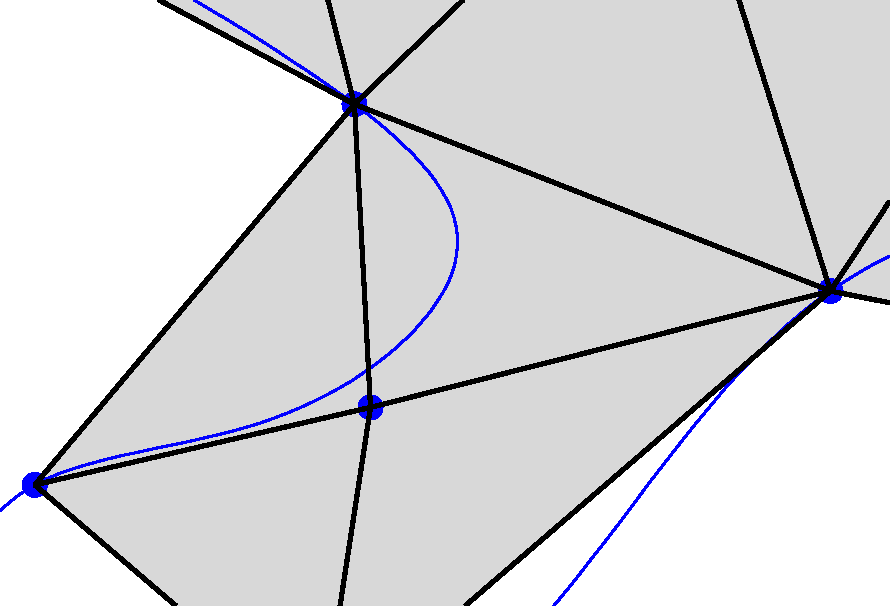
\includegraphics[width=0.3\textwidth]{untangling/linear} &
  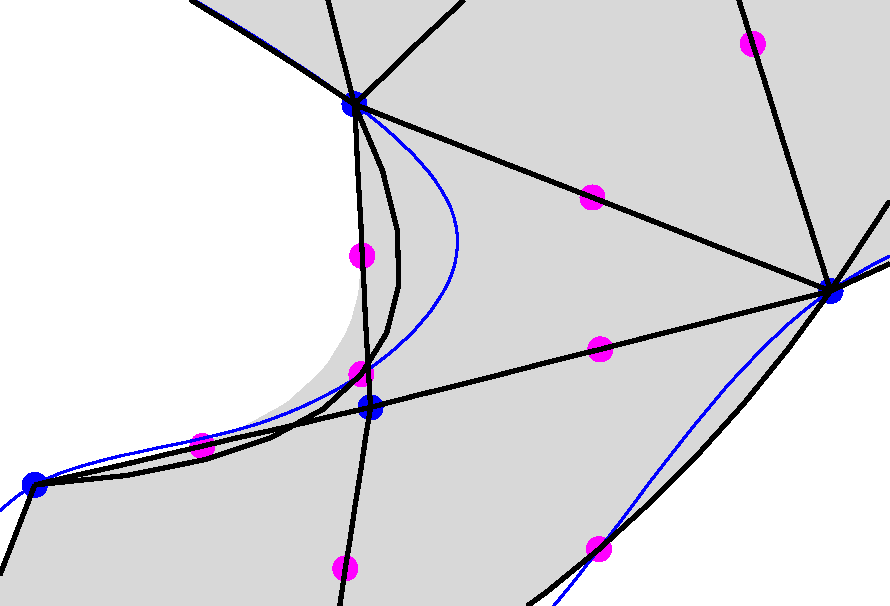
\includegraphics[width=0.3\textwidth]{untangling/p2_bad} &
  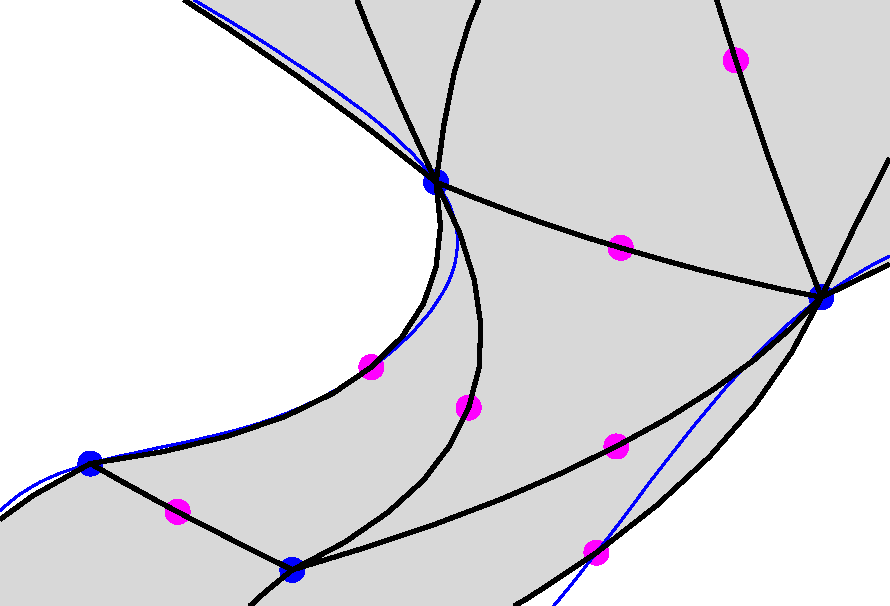
\includegraphics[width=0.3\textwidth]{untangling/p2}\\
  First-order mesh & High-order vertices &\textbf{Untangling}
  \end{tabular}
\end{center}
\caption{Straight sided mesh (left) basic curvilinear (quadratic)
mesh with tangled elements (center) and untangled mesh (right).
\label{fig:untangling}}
\end{figure}

To this end, elements whose scaled Jacobian lies outside the
range $[J_{\min}, J_{\max}]$ are considered as bad elements. Two
optimization passes are defined. In the first pass, two
contributions are included: the square of the node displacement
(see Section~\ref{sec:problem-def}) and a moving log barrier against
the minimum of the scaled Jacobian, with $J_{\min}$ as target value
and $0$ as critical value. In the second pass, the moving barrier
against the minimum scaled Jacobian is replaced by a fixed barrier
on the minimum scaled Jacobian plus a moving barrier on the maximum
scaled Jacobian with $J_{\max}$ as target value.


The high-order mesh optimizer is accessible from the ``High-order
tools'' window in Gmsh's graphical interface. The parameters are
as follows:

\begin{itemize}
\item \texttt{Target Jacobian range} corresponds to $J_{\min}$ and
$J_{\max}$.
\item \texttt{Number of layers} is the maximum number of layers
around a bad element to be included in a patch (see \texttt{minLayers}
in Section~\ref{sec:patch-selec}).
\item \texttt{Distance factor} controls the distance criterion
for the creation of patches (see Section~\ref{sec:patch-selec}). The
factor is multiplied by the maximum distance, among all high-order
nodes in a bad element, between the node and the corresponding location
in a straight-sided version of the bad element.
\item \texttt{Boundary nodes} determines whether the boundary nodes
are fixed or are allowed to move along the corresponding boundary
in case a CAD model is available.
\item \texttt{Weight on node displacement} is the relative weight
of the node displacement contribution compared to the Jacobian
contributions.
\item \texttt{Maximum number of iterations} is the maximum number
of iterations in the Conjugate Gradient algorithm (see
\texttt{maxOptIter} in Section~\ref{sec:input-param}).
\item \texttt{Max. number of barrier updates} is the maximum number
of times the log barriers are moved (see \texttt{maxParamUpdates} in
Section~\ref{sec:input-param}).
\item \texttt{Strategy} determines the strategy for the treatment of
patches (see Sections~\ref{sec:strategy} and~\ref{sec:patch-selec}).
\item \texttt{Max. number of blob adaptation iter.},
\texttt{Num. layer adaptation factor} and
\texttt{Distance adaptation factor} control the adaptation of the
patch size in the ``adaptive one-by-one'' strategy (see
\texttt{maxPatchAdapt}, \texttt{maxLayersAdaptFact} and
\texttt{distanceAdaptFact} in Section~\ref{sec:patch-selec}).
\end{itemize}

These options are likely to change as the high-order mesh
optimizer is being further developed.


\subsection{Mesh Quality Optimizer}

The mesh quality optimizer aims to improve the quality of meshes,
as measured by the ``inverse condition number'' quality metric.
The elements below a quality threshold are marked as bad, and a
unique optimization pass includes two contributions: the square
of the node displacement (see Section~\ref{sec:problem-def}) and
a moving log barrier against the minimum of the quality measure.

The mesh quality optimizer is only accessible through Gmsh's API
in C++ or Python. It is launched by the function
\texttt{MeshQualityOptimizer}, that take as arguments a pointer to
an instance of GModel and a structure \texttt{MeshQualOptParameters}
as follows:
\begin{verbatim}
struct MeshQualOptParameters {
  bool onlyValidity;
  bool excludeQuad, excludeHex, excludePrism, excludeBL;
  double minTargetIdealJac;
  double minTargetInvCondNum;
  double weight;
  int nbLayers;
  int dim;
  int maxOptIter;
  int maxBarrierUpdates;
  bool onlyVisible;
  double distanceFactor;
  bool fixBndNodes;
  int strategy;
  int maxPatchAdapt;
  int maxLayersAdaptFact;
  double distanceAdaptFact;
  int SUCCESS;
  double minIdealJac, maxIdealJac;
  double minInvCondNum, maxInvCondNum;
  double CPU;

  MeshQualOptParameters ()
    : onlyValidity(false), excludeQuad(false),
      excludeHex(false), excludePrism(false), excludeBL(false),
      minTargetIdealJac(0.1), minTargetInvCondNum(0.1),
      weight(1.), nbLayers(6), dim(3), maxOptIter(300),
      maxBarrierUpdates(50), onlyVisible(true),
      distanceFactor(12), fixBndNodes(false), strategy(0),
      maxPatchAdapt(3), maxLayersAdaptFact(2),
      distanceAdaptFact(2.), CPU(0.), minIdealJac(0.),
      maxIdealJac(0.), minInvCondNum(0.), maxInvCondNum(0.),
      SUCCESS(-1)
  {
  }
};
\end{verbatim}

Many parameters correspond directly to those of
\texttt{MeshOptParameters} and \texttt{PatchDef} described in
Sections~\ref{sec:input-param} and~\ref{sec:patch-selec}. The
differences are:
\begin{itemize}
\item The boolean \texttt{onlyValidity} forces the optimizer to
use the ``ideal Jacobian'' of the element instead of the inverse
condition number when set to \texttt{true}.
\item The booleans \texttt{excludeQuad}, \texttt{excludeHex} and
\texttt{excludePrism} make it possible to exclude from the
optimization the quadrangular, prismatic and hexahedral elements
respectively.
\item The boolean \texttt{excludeBL}, when set to \texttt{true},
excludes the boundary layer elements from the optimisation.
\item The field \texttt{minTargetIdealJac} sets the target value
for the minimum ideal Jacobian (if \texttt{onlyValidity} is
\texttt{true}).
\item The field \texttt{minTargetInvCondNum} sets the target
value for the inverse condition number (if \texttt{onlyValidity}
is \texttt{false}).
\item The field \texttt{weight} is the relative weight of the node
displacement contribution compared to the inverse condition number
or Jacobian contribution.
\item The field \texttt{strategy} determines the strategy in the
manner of the patch selection options in
Section~\ref{sec:patch-selec}: $0$ corresponds to
\texttt{STRAT\_DISJOINT} with \texttt{weakMerge} set to
\texttt{false}, $1$ corresponds to \texttt{STRAT\_ONEBYONE}
and $2$corresponds to \texttt{STRAT\_DISJOINT} with
\texttt{weakMerge} set to \texttt{true}.
\item The fields \texttt{minIdealJac} and \texttt{maxIdealJac}
return the extrema of the ideal Jacobian in the output mesh
(if \texttt{onlyValidity} is \texttt{true}).
\item The fields \texttt{minInvCondNum} and
\texttt{maxInvCondNum} return the extrema of the inverse condition
number in the output mesh (if \texttt{onlyValidity} is
\texttt{false}).
\end{itemize}

These options are likely to change as the mesh quality optimizer
is being further developed.

%-----------------------------------------
%\clearpage
%\bibliographystyle{abbrv}
%\bibliography{D41-30b}


\begin{thebibliography}{2}

\bibitem{bounds-jcp}
A.~Johnen, J.-F.~Remacle, and C.~Geuzaine.
\newblock Geometrical validity of curvilinear finite elements.
\newblock {\em J. Comput. Phys.}, 233:359--372, 2013.

\bibitem{untangling-jcp}
T.~Toulorge, C.~Geuzaine, J.-F. Remacle, and J.~Lambrechts.
\newblock Robust untangling of curvilinear meshes.
\newblock {\em J. Comput. Phys.}, 254:8--26, 2013.

\end{thebibliography}


\end{document}
